\documentclass{rapport}
\usepackage[utf8]{inputenc}

\usepackage{pifont} % Pour les symboles appelés par la macro \ding
\usepackage{url} % Comme son nom l'indique, pour les url...

\usetikzlibrary{positioning} % Bibliothèque tikz pour positionner des nœuds relativement à d'autres

\usepackage[colorlinks, citecolor=red!60!green, linkcolor=blue!60!green, urlcolor=magenta]{hyperref} % Pour que les liens soient cliquables. Les options permettent de mettre les liens en couleur.

\usepackage{algorithm}
\usepackage{algo}
\usepackage{colorationSyntaxique}


% Pour un rapport en français 
% \usepackage[francais]{babel} % Commenter pour un rapport en anglais
% \renewcommand\bibsection{\section*{Bibliographie}} % Commenter pour un rapport en anglais

\englishTitlePage % Décommenter pour une page de titre en anglais


\pagestyle{fancy}
\renewcommand{\sectionmark}[1]{\markboth{\thesection.\ #1}{}}
\fancyfoot{}

\fancyhead[LE]{\textsl{\leftmark}}
\fancyhead[RE, LO]{\textbf{\thepage}}
\fancyhead[RO]{\textsl{\rightmark}}

\def\Latex{\LaTeX\xspace}
\def\etc{\textit{etc.}\xspace}



\title{Hardware Performance Counters}
\author{Francois Flandin}
\supervisor{Sid Touati}
\date{Second semestre de l'année 2024-2025}

\universityname{Université Côte d'Azur} % Nom de l'université.
\type{TER} % Type de document
\formation{Master Informatique} % Nom de la formation

% Retrouver les autres options possibles dans le document rapport.pdf

\begin{document}

  \maketitle

  \begin{abstract}
    Calmos le ramoloss, l'abstract c'est pas pour tout de suite
  \end{abstract}

  \clearpage
  \tableofcontents
  \clearpage
  \section{Introduction}
  If you wish to explore the details of the work done for the project, the project's code is hosted on GitHub at https://github.com/omelette-bio/projet-tutorat-s2-m1

  \clearpage


  \section{Checking CPU capabilities : the \texttt{CPUID} instruction}

  En gros sur les archi x86 il existe une instruction CPUID qui lit des registres pour donner des infos sur le CPU, donc marque, vendeur, memoire adressable, mais aussi les capacites en termes de CMP.
  L'instruction CPUID se divise en feuilles et en sous-feuilles, permettant de lire differentes informations, repartie dans 4 registres eax, ebx, ecx, edx, 
  par exemple, la feuille 0x80000008, dans le registre eax sur intel donne des informations sur la nombre d'adresses adressables par notre cpu. 
  On utilisera la notation \texttt{CPUID[LEAF].REG} pour noter les informations obtentibles avec la commande \texttt{CPUID}, sous la feuille \texttt{LEAF}, 
  dans le registre \texttt{REG}.

  
  


  	\section{Hardware Performance Monitoring on INTEL CPUs}

  	\subsection{\texttt{CPUID} sous intel cpus}

	\texttt{CPUID[0x0A].EAX} nous donne toutes les informations necessaires relatives aux compteurs materiels de performance sous intel cpu, decortiquons son contenu
	\begin{description}
		\item [bits {[7:0]}] donnent le numero version du Architectural Performance Monitoring supporte
		\item [bits {[15:8]}] donnent le nombre de MSR par coeur logique
		\item [bits {[23:16]}] donnent la taille en bits des registres \texttt{IA32\_PMCx}
		\item [bits {[31:24]}] donnent le nombre d'evenements architecturaux
	\end{description}

	\subsection{Performance Monitoring MSRs on Intel cpus}

  	\begin{figure}[H]
		\centering
		\makebox[\textwidth]{
		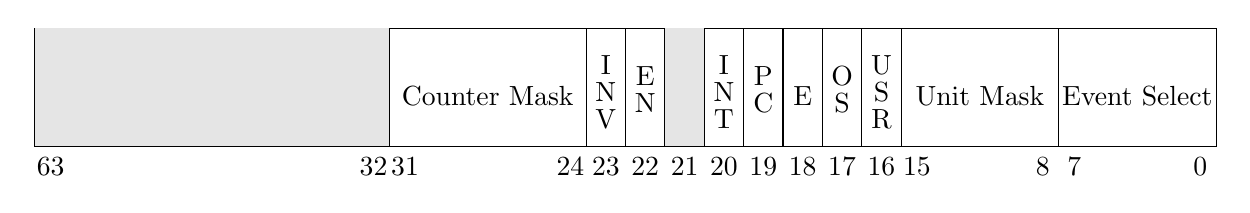
\begin{tikzpicture}
			% Draw the main box
			\draw (0,0) rectangle (15,1.5);

			\node[anchor=south] at (0.2,-0.5) {63};
			\fill[gray!20] (0,0) rectangle (4.5,1.5);
			\node[anchor=south] at (4.3,-0.5) {32};

			\draw (4.5,0) -- (4.5,1.5);

			\node[anchor=south] at (4.7,-0.5) {31};
			\node[anchor=south] at (5.75,0.4)  {Counter Mask};
			\node[anchor=south] at (6.8,-0.5) {24};

			\draw (7,0) -- (7,1.5);

			\node[anchor=south] at (7.25,0.1) {\shortstack{I\\N\\V}};
			\node[anchor=south] at (7.25,-0.5) {23};

			\draw (7.5,0) -- (7.5,1.5);

			\node[anchor=south] at (7.75,0.3) {\shortstack{E\\N}};
			\node[anchor=south] at (7.75,-0.5) {22};

			\draw (8,0) -- (8,1.5);

			\fill[gray!20] (8,0) rectangle (8.5,1.5);
			\node[anchor=south] at (8.25,-0.5)	{21};

			\draw (8.5,0) -- (8.5,1.5);

			\node[anchor=south] at (8.75,0.1)	{\shortstack{I\\N\\T}};    		
			\node[anchor=south] at (8.75,-0.5)	{20};

			% Draw sub-boxes
			\draw (9,0) -- (9,1.5);

			\node[anchor=south] at (9.25,0.3) {\shortstack{P\\C}};
			\node[anchor=south] at (9.25,-0.5) {19};

			\draw (9.5,0) -- (9.5,1.5);

			\node[anchor=south] at (9.75,0.4) {E};
			\node[anchor=south] at (9.75,-0.5) {18};

			\draw (10,0) -- (10,1.5);

			\node[anchor=south] at (10.25,0.3) {\shortstack{O\\S}};
			\node[anchor=south] at (10.25,-0.5) {17};

			\draw (10.5,0) -- (10.5,1.5);

			\node[anchor=south] at (10.75,0.1)	{\shortstack{U\\S\\R}};    		
			\node[anchor=south] at (10.75,-0.5)	{16};

			\draw (11,0) -- (11,1.5);

			\node[anchor=south] at (11.2,-0.5)	{15};
			\node[anchor=south] at (12,0.4)  {Unit Mask};
			\node[anchor=south] at (12.8,-0.5)  {8};

			\draw (13,0) -- (13,1.5);

			\node[anchor=south] at (13.2,-0.5)  {7};
			\node[anchor=south] at (14,0.4)	{Event Select};
			\node[anchor=south] at (14.8,-0.5)	{0};
		\end{tikzpicture}
   		}
   	\label{fig:figure1}
   	\caption{Bit Repartition of \texttt{IA32\_PERFEVTSELx}}
	\end{figure}

  \section{Hardware Performance Monitoring on AMD CPUs}

  	\begin{figure}[H]
        \centering
        \makebox[\textwidth]{
    	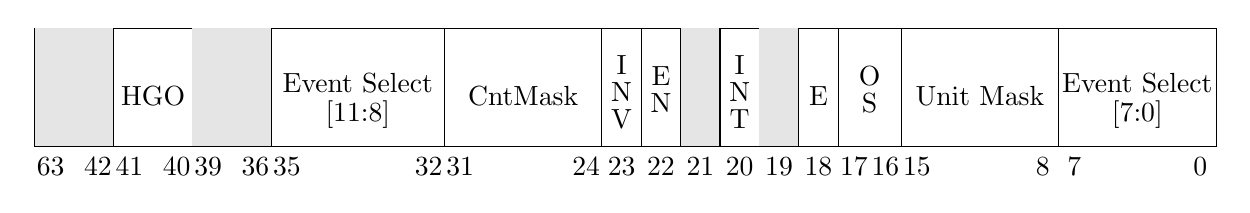
\begin{tikzpicture}
    		% Draw the main box
    		\draw (0,0) rectangle (15,1.5);
    
    		% Draw sub-boxes
    		\draw (0,0) -- (0,1.5); % debut zone reservee
    
    		\node[anchor=south] at (0.2,-0.5) {63};
    		\fill[gray!20] (0,0) rectangle (1,1.5);
    		\node[anchor=south] at (0.8,-0.5) {42};
    
    		\draw (1,0) -- (1,1.5);
        
            \node[anchor=south] at (1.2,-0.5)	{41};
    		\node[anchor=south] at (1.5,0.4)	{HGO};    		
    		\node[anchor=south] at (1.8,-0.5)	{40};
        
            \draw (2,0) -- (2,1.5);
            
            \node[anchor=south] at (2.2,-0.5)	{39};
            \fill[gray!20] (2,0) rectangle (3,1.5);
            \node[anchor=south] at (2.8,-0.5)	{36};
            
            \draw (3,0) -- (3,1.5);
    
            \node[anchor=south] at (3.2,-0.5)	{35};
    		\node[anchor=south] at (4.1,0.1)	{\shortstack{Event Select\\{[11:8]}}};
    		\node[anchor=south] at (5,-0.5)	{32};
    
            \draw (5.2,0) -- (5.2,1.5);
            
            \node[anchor=south] at (5.4,-0.5)	{31};
    		\node[anchor=south] at (6.2,0.4)	{CntMask};
    		\node[anchor=south] at (7,-0.5)	{24};
      
            \draw (7.2,0) -- (7.2,1.5);
    
    		\node[anchor=south] at (7.45,-0.5) {23};
    		\node[anchor=south] at (7.45,0.1)  {\shortstack{I\\N\\V}};
    
    		\draw (7.7,0) -- (7.7,1.5);
    
    		\node[anchor=south] at (7.95,-0.5) {22};
    		\node[anchor=south] at (7.95,0.3)  {\shortstack{E\\N}};
    
    		\draw (8.2,0) -- (8.2,1.5);
    
    		\node[anchor=south] at (8.45,-0.5) {21};
    		\fill[gray!20] (8.2,0) rectangle (8.7,1.5);
    
    		\draw (8.7,0) -- (8.7,1.5);
    
            \node[anchor=south] at (8.95,-0.5)	{20};
    		\node[anchor=south] at (8.95,0.1)  {\shortstack{I\\N\\T}};
    
    		\draw (9.2,0) -- (9.2,1.5);
    
    		\node[anchor=south] at (9.45,-0.5)	{19};
    		\fill[gray!20] (9.2,0) rectangle (9.7,1.5);
    
    		\draw (9.7,0) -- (9.7,1.5);
    
    		\node[anchor=south] at (9.95,-0.5) {18};
    		\node[anchor=south] at (9.95,0.4)  {E};
    
    		\draw (10.2,0) -- (10.2,1.5);
    
    		\node[anchor=south] at (10.4,-0.5)	{17};
    		\node[anchor=south] at (10.6,0.3)	{\shortstack{O\\S}};    		
    		\node[anchor=south] at (10.8,-0.5)	{16};
    
    		\draw (11,0) -- (11,1.5);
    
    		\node[anchor=south] at (11.2,-0.5)	{15};
    		\node[anchor=south] at (12,0.4)  {Unit Mask};
    		\node[anchor=south] at (12.8,-0.5)  {8};
    
    		\draw (13,0) -- (13,1.5);
    
    		\node[anchor=south] at (13.2,-0.5)  {7};
    		\node[anchor=south] at (14,0.1)	{\shortstack{Event Select\\{[7:0]}}};
    		\node[anchor=south] at (14.8,-0.5)	{0};
    	\end{tikzpicture}
	   }
	   \label{fig:figure1}
	   \caption{Bit Repartition of \texttt{MSRC001\_020[A,8,6,4,2,0]}}
	\end{figure}

  
	
  \pageblanche
  \bibliographystyle{apalike-fr}
  \bibliography{biblio}

\end{document}
